\section{Validation}

To validate our implementation of the stochastic simulation model, the 3 region problem previously solved using differential equations, is now solved using the stochastic model.

\begin{figure}[H]
	\centering
	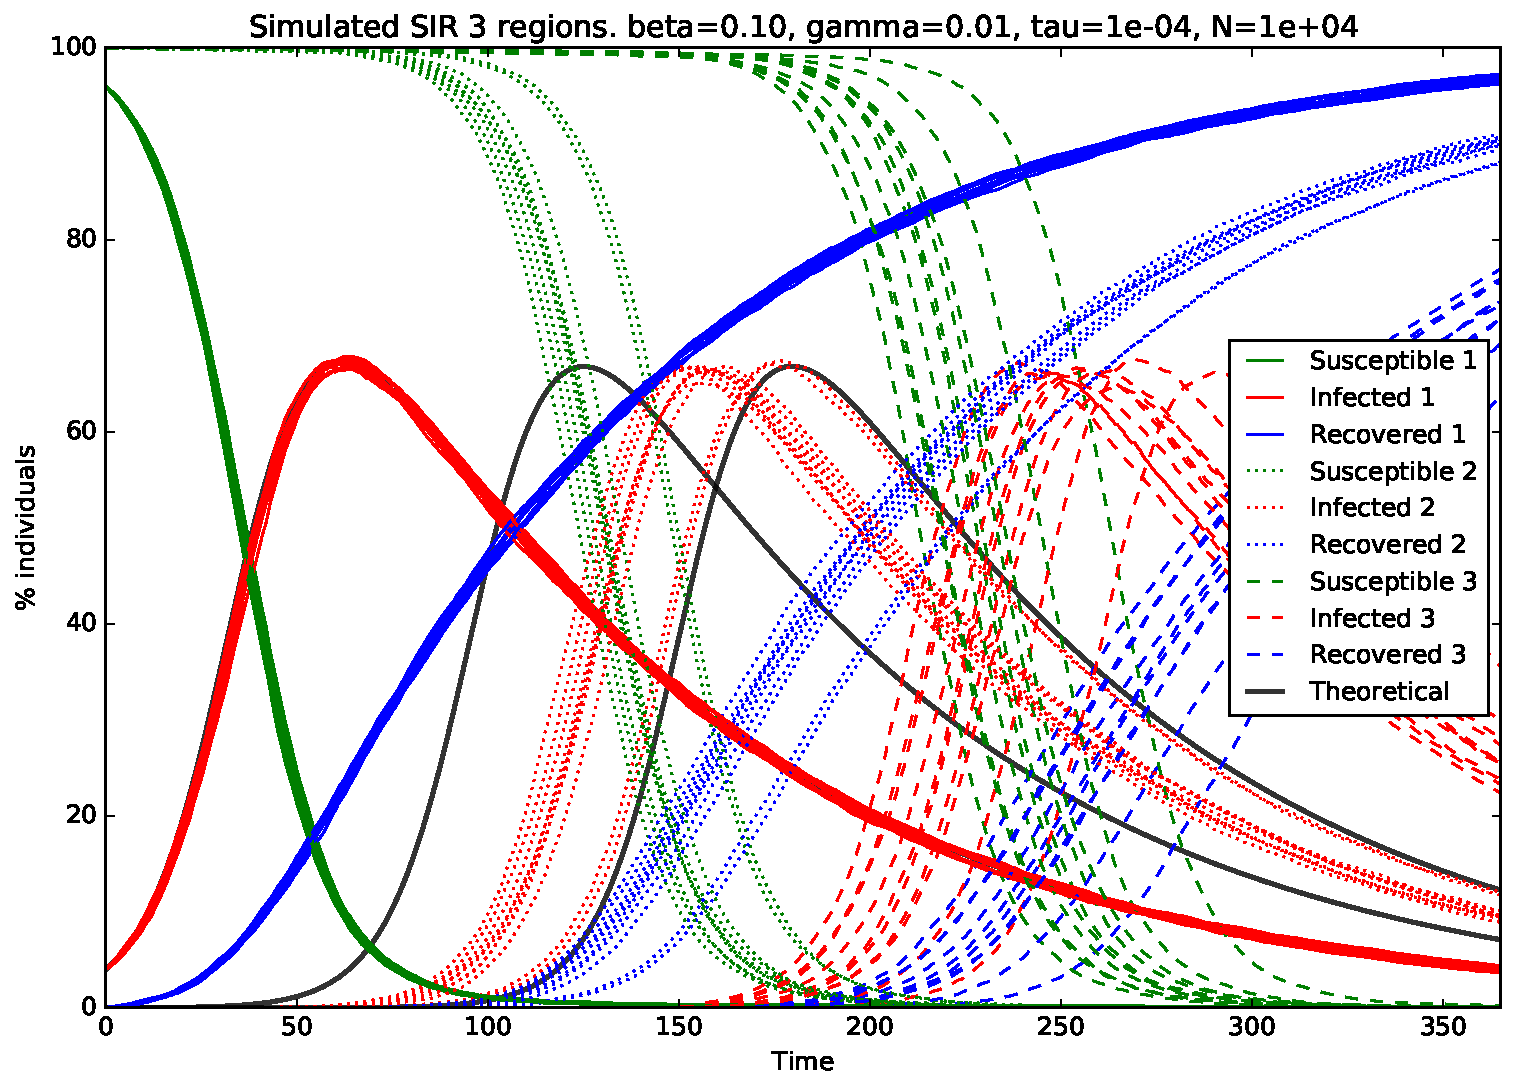
\includegraphics[width= 1.0 \linewidth]{plots/sir_three_region_sim_10000.pdf}
	\caption{10 solutions using the stochastic simulation model, on the same 3-region problem as in the theoretical case.}
	\label{fig:sir_three_region_sim_10000}
\end{figure}

Figure \ref{fig:sir_three_region_sim_10000} shows a big discrepancy between the solution obtained using differential equations and the those obtained using stochastic simulation. This is most likely because the differential equation model allows for transferring people partially, . This means regions that has a very low probability of getting infected early in the stochastic model, starts their infection immediately in the differential equation model. This hypothesis can be validated by increasing the number of people in each region (N), as this will cause the discreteness of the stochastic model to be less important. The result of this can be seen in figure \ref{fig:sir_three_region_sim_1000000}. 

\begin{figure}[H]
	\centering
	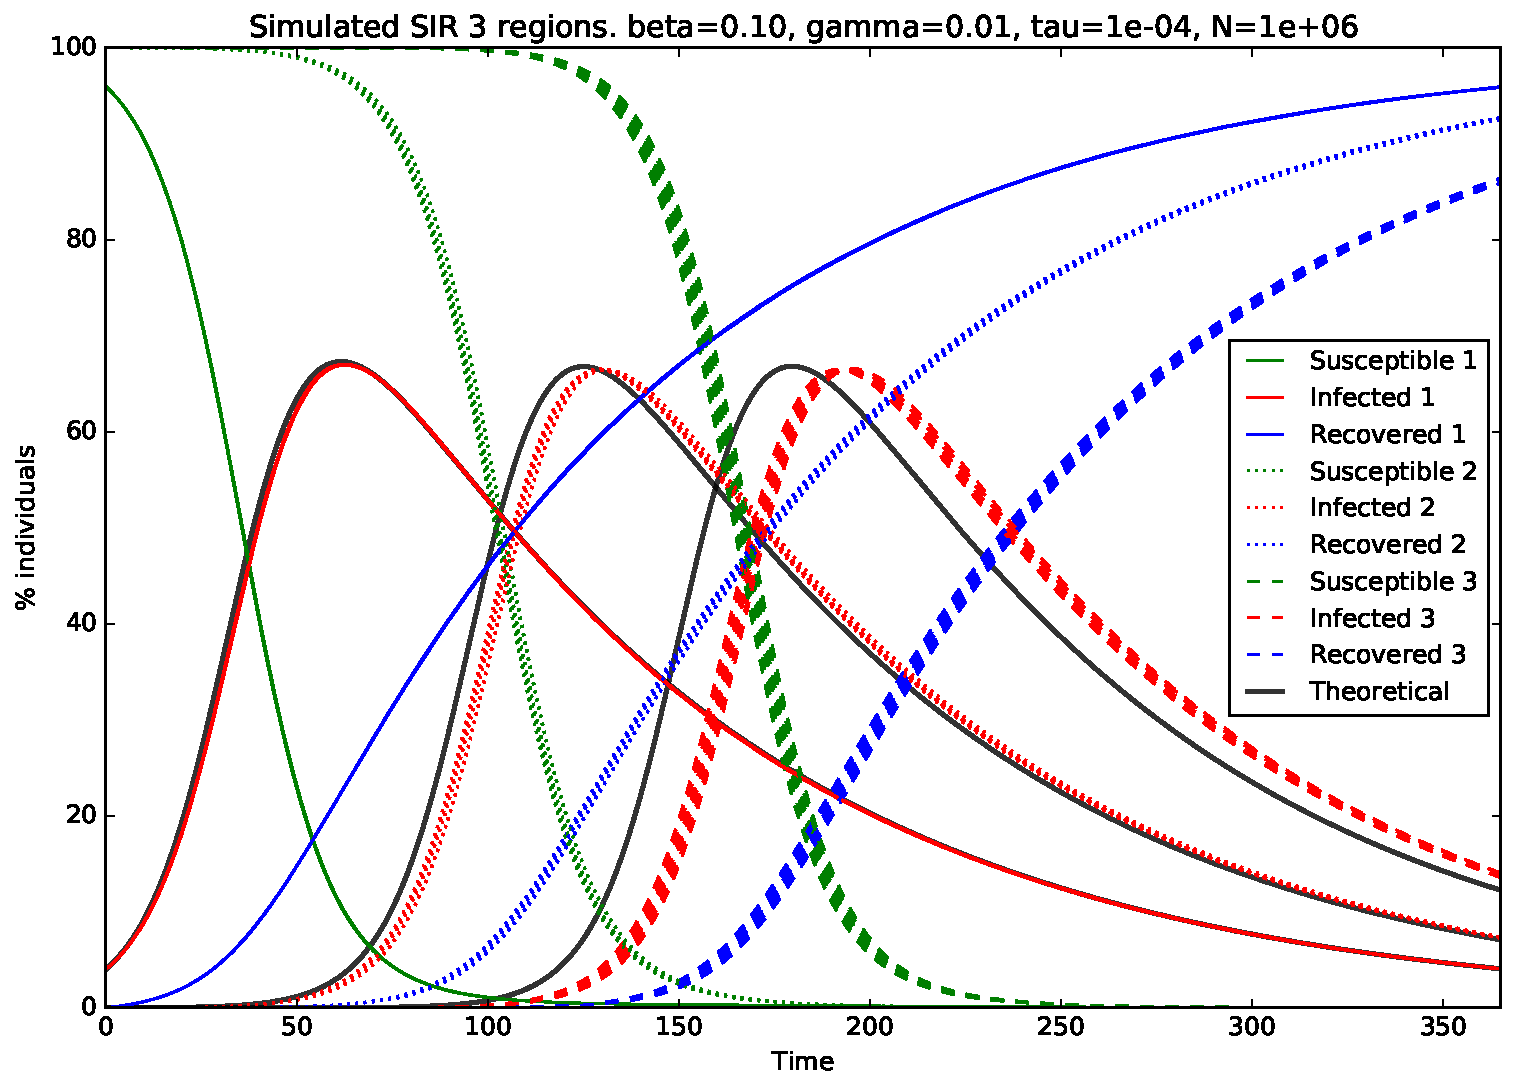
\includegraphics[width= 1.0 \linewidth]{plots/sir_three_region_sim_1000000.pdf}
	\caption{10 solutions using the stochastic simulation model, on the same 3-region problem as in the theoretical case.}
	\label{fig:sir_three_region_sim_1000000}
\end{figure}

As seen in figure \ref{fig:sir_three_region_sim_1000000} having more people results a much smaller discrepancy. This discrepancy caused by using a discrete model is not necessarily a failure of the stochastic model, but rather it is the differential equation model that overestimates the infection start for initially healthy regions.
